% id: 63-c5
% book: 개념원리 중학 3-2 · 06 원의 현
% section: 핵심문제 익히기
% figure: crop:fig-63-c5.png
% answer: $3\sqrt{5}\mkern3mu \mathrm{cm}$
% answer_source: 답지
% variant_level: 0 (원본 전사)
% 이 파일은 build.mjs 가 items.json 에서 만든다. 고칠 때는 items.json 을 고친다.
\smash{\raisebox{1.5mm}{\dmkichul{개념원리 중학 3-2 63쪽 확인 5}}}
\noindent\begin{minipage}[t]{0.58\linewidth}\vspace{0pt}\raggedright 오른쪽 그림과 같이 반지름의 길이가 $9\mkern3mu \mathrm{cm}$인 원~$\pt{O}$에서 $\seg{AB}\perp\seg{OM}$, $\seg{CD}\perp\seg{ON}$이고 $\seg{AB}=\seg{CD}=12\mkern3mu \mathrm{cm}$일 때, $\seg{OM}$의 길이를 구하시오.\end{minipage}\hfill\begin{minipage}[t]{0.4\linewidth}\vspace{0pt}\centering \setlength{\dmfigw}{68.2pt}\ifdim\dmfigw>\linewidth\setlength{\dmfigw}{\linewidth}\fi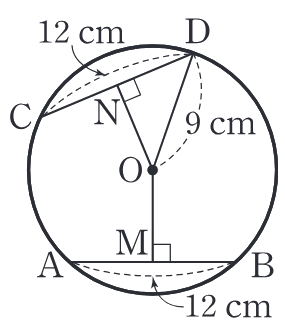
\includegraphics[width=\dmfigw]{figures/fig-63-c5.png}\end{minipage}\par
